% Section 5: results around Tables T2–T6.
% Evidence: VANET protocol §4c (T2), §8.6–§8.7 (pilot, ablation), §8.8 (gate, T3), §8.1a/§8.6/§8.10 (T4), §8.9–§8.10 (T5, T5b), §8.11 (T6).
% Figures F2–F5 in ../figures/ are produced by VANET/.../paper2_revision/make_r2_figures.py from the same records.
\section{Results}
\label{sec:results}

Section~\ref{sec:concealed} re-measures the submitted safety table and shows, with the same checkpoints, which of its conclusions the defects produced. Sections~\ref{sec:agreement} and~\ref{sec:collapse} report the first runs under the corrected contract: the pilot (two CALM seeds, two entropy-only seeds, one unconstrained MADDPG seed, one QMIX-CALM seed) and the unweighted-prior ablation, all randomly initialised except where a prior is named. Section~\ref{sec:anchor} is the pre-registered isolation of the anchor, Section~\ref{sec:prior} the frozen-prior control on the same episodes, and Section~\ref{sec:reward} the training reward, labelled as such. Unless stated otherwise, simulator figures are under lane-change mode 512 and sampled execution, entropies are normalised by $\log 5$, and ``exits'' is the share of exit-assigned agents that left by a ramp.

\subsection{What the defects concealed}
\label{sec:concealed}

\paragraph{The exit column.}
Table~\ref{tab:t2_table3} replays the submitted Table~III: the same Week~5 checkpoints, the same legacy observation contract and action order, the same episode seeds, 100 episodes per method, with the evaluator's agent lifecycle repaired (D4). Average speed and proximity events reproduce the submitted values to full floating-point precision for every method, because both are computed over every vehicle present in the simulation whatever the tracking set. Only the exit column changed. All five agents departed in every one of the 500 episodes, and once the three exit agents were tracked rather than one, CALM's exit success rose from 33.3\,\% to 100\,\%, QMIX-CALM's from 26.7 to 81.0, entropy-only's from 20.0 to 60.0, DAgger's from 7.7 to 28.3 and GAIL's from 6.7 to 20.0. The submitted ``exactly one exit per episode'' for CALM was the exit of the one tracked agent in each of the 100 episodes; the other two exit agents exited in every episode as well. The ordering of the methods is unchanged; every sentence the submitted paper wrote about the magnitudes is not. Collisions, defined as teleports, were zero in every cell before and after the repair; with all five agents tracked that is the stronger statement. The slow policies' behavioural reading stands: DAgger at 11.0\,m/s and GAIL at 8.1\,m/s rarely exit and accumulate thousands of proximity events per episode. These are measurements of the defective pipeline and are not used as comparators for anything below.

\paragraph{Baseline identities.}
Table~\ref{tab:t3_gate} evaluates the pilot and ablation checkpoints under all four combinations of lane-change control (SUMO default, mode 512) and execution rule (greedy, sampled), beside the three reference policies, 50 episodes per seed on the pilot's episode seeds. Under SUMO's default lane changing and greedy execution, CALM with the class-balanced prior is the constant Lane\_Right policy to the decimal: 100\,\% exits, 25.3\,m/s, 7.5 proximity events per agent-km, 555 commanded rightward moves and none by SUMO, lane-0 share 0.96; its selected-action entropy is 0.01. CALM with the unweighted prior is constant Maintain, which under this mode is also the SUMO-default policy: 27.2\,m/s, 6.2 per km, zero commanded moves and 553 made by SUMO. The two greedy anchored policies that the pilot evaluated are therefore two constant policies, and the submitted paper's safety profile (full exits, highest speed, fewest near-misses, no collisions) is the profile of whichever constant action the prior's class weighting put first (Section~\ref{sec:collapse}). The step log confirms it: all ten class-balanced CALM agents select Lane\_Right on at least 99\,\% of steps, 94\,\% of those decisions being boundary no-ops in lane~0; all ten unweighted CALM agents select Maintain on 100\,\%.

\paragraph{Execution-rule dependence.}
Under the rule CALM trains with, the same checkpoints are different policies. Sampled class-balanced CALM has per-state entropy 0.71 over the states it visits and selected-action entropy 0.72 against 0.01 greedy, and uses all four non-Lane\_Left actions (Lane\_Right 54\,\%, Maintain 25\,\%, Decelerate 11\,\%, Accelerate 10\,\%). Definition~1 is thus preserved in the simulator as well as on the validation split; ``greedy CALM is a constant policy'' is true and ``CALM has no behavioural diversity'' is not. The diversity has a price on every safety column: speed 25.3 to 12.1\,m/s, exits 100 to 80\,\%, proximity 7.5 to 37.2 per agent-km. The pilot's safety advantages belong to the greedy constant policy, not to the stochastic policy that was trained. Greedy and sampled figures are never placed in one comparison in the rest of this paper.

\paragraph{Whose lane changes.}
Under SUMO's default mode, 70\,\% of unconstrained MADDPG's and 48\,\% of entropy-only's rightward exit-lane moves were SUMO's, and a policy that commands nothing exits in every episode. Under mode 512 the same do-nothing policies (constant Maintain, SUMO default, greedy unweighted CALM) exit in 7\,\% of cases, those in which the first exit agent happened to depart in lane~0, and otherwise strand at the end of the segment at 8.4\,m/s with 681 proximity events per agent-km. Greedy unconstrained MADDPG drops from 100 to 33\,\% (one exit agent, 84 commanded moves), entropy-only from 82 to 50\,\% greedy and from 80 to 65\,\% sampled. Class-balanced CALM keeps 100\,\% greedy and 78\,\% sampled, every move commanded, and QMIX-CALM keeps 100\,\%: these two methods' exits were the policy's under both modes, which is what lets Sections~\ref{sec:anchor}--\ref{sec:prior} compare them with the prior. For every policy whose commanded share was low, exit success under the default mode measured SUMO.

\paragraph{Collisions.}
Across the 2{,}100 gate episodes, teleports and direct collisions were both zero in every run, including the stranded reference policies under mode 512. Adding the 500 re-measured legacy episodes, the 400 pilot and ablation episodes, the 800 Option~B episodes, the 200 frozen-prior episodes and the 100 of B1's re-evaluation in the sections below, no agent teleported in any of the roughly 4{,}100 evaluation episodes of this paper, and no direct collision was recorded in the 3{,}200 in which the collision list was read. Mode 512 keeps SUMO's car-following and gap enforcement, so a commanded lane change is still refused when the gap is unsafe. Zero collisions is what this simulator does for every policy, and no result in this paper rests on it. Exposure normalisation (per agent-km) changes little in the ordering of policies but much in the magnitudes: the sampled policies' proximity is three to five times their greedy counterparts', and the stranded policies are two orders of magnitude worse than any trained policy.

\begin{table*}[t]
\centering
\caption{Submitted Table III (historical: defective pipeline, legacy observation contract) beside its re-measurement with the agents tracked for the whole episode (protocol \S4c; same checkpoints, same legacy contract, 100 episodes per method). The submitted exit column counted only agents still tracked after step 1.}
\label{tab:t2_table3}
\footnotesize
\resizebox{\textwidth}{!}{%
\begin{tabular}{lccccccc}
\toprule
\textbf{Method} & \textbf{Exit \% (subm.)} & \textbf{Exit \% (re-meas.)} & \textbf{Speed m/s (subm.)} & \textbf{Speed m/s (re-meas.)} & \textbf{Prox./ep (subm.)} & \textbf{Prox./ep (re-meas.)} & \textbf{Collisions \%} \\
\midrule
CALM (class-balanced prior) & 33.3 & 100.0 & 25.8 $\pm$ 1.2 & 25.8 $\pm$ 1.2 & 42.5 & 42.5 & 0.0 \\
QMIX-CALM ($n=5$) & 26.7 & 81.0 & 19.7 $\pm$ 6.9 & 19.7 $\pm$ 6.9 & 220.9 & 220.9 & 0.0 \\
Entropy-only ($\alpha=0.01$) & 20.0 & 60.0 & 16.3 $\pm$ 6.1 & 16.3 $\pm$ 6.1 & 685.4 & 685.4 & 0.0 \\
DAgger & 7.7 & 28.3 & 11.0 $\pm$ 3.6 & 11.0 $\pm$ 3.6 & 3150.5 & 3150.5 & 0.0 \\
GAIL & 6.7 & 20.0 & 8.1 $\pm$ 2.2 & 8.1 $\pm$ 2.2 & 2563.8 & 2563.8 & 0.0 \\
\bottomrule
\end{tabular}}
\vspace{1mm}
\parbox{\textwidth}{\scriptsize Historical record only: these checkpoints were trained on raw SUMO features with an unpermuted action order (protocol \S1) and are not comparators for any corrected-contract result. Collision rate as submitted = fraction of episodes with $\geq 1$ teleport; 0 in every cell.}
\end{table*}

\begin{table*}[t]
\centering
\caption{Diagnostic gate (protocol \S8.8): the same checkpoints evaluated under SUMO's default lane changing and under policy-attributable lane changes (\texttt{agent\_lane\_change\_mode=512}), with greedy and sampled execution, beside the three reference policies. 50 episodes per seed; zero direct collisions and zero teleports in every cell.}
\label{tab:t3_gate}
\footnotesize
\resizebox{\textwidth}{!}{%
\begin{tabular}{lcccccccc}
\toprule
\textbf{Contract, execution: policy} & \textbf{$n$} & \textbf{Exit \%} & \textbf{Speed m/s} & \textbf{Prox./agent-km} & \textbf{$H$ per-state} & \textbf{$H$ selected} & \textbf{Lane changes L / R} & \textbf{Lane-0 share} \\
\midrule
SUMO default, greedy: CALM (class-balanced prior) & 100 & 100.0 & 25.3 & 7.5 & 0.65 & 0.01 & 555 / 0 & 0.96 \\
SUMO default, greedy: CALM (unweighted prior) & 100 & 100.0 & 27.2 & 6.2 & 0.44 & 0.00 & 0 / 553 & 0.50 \\
SUMO default, greedy: Entropy-only ($\alpha=0.01$) & 100 & 82.3 & 18.9 & 56.2 & 0.36 & 0.74 & 280 / 260 & 0.62 \\
SUMO default, greedy: MADDPG, no prior & 50 & 100.0 & 26.8 & 11.7 & 0.36 & 0.81 & 84 / 193 & 0.52 \\
SUMO default, greedy: QMIX-CALM ($n=5$) & 50 & 100.0 & 24.4 & 10.6 & -- & 0.33 & 278 / 0 & 0.96 \\
SUMO default, greedy: Constant Maintain & 100 & 100.0 & 27.2 & 6.2 & 0.00 & 0.00 & 0 / 553 & 0.50 \\
SUMO default, greedy: Constant Lane\_Right & 100 & 100.0 & 25.3 & 7.5 & 0.00 & 0.00 & 555 / 0 & 0.96 \\
SUMO default, greedy: SUMO default (no commands) & 100 & 100.0 & 27.2 & 6.2 & -- & 0.00 & 0 / 553 & 0.50 \\
\midrule
SUMO default, sampled: CALM (class-balanced prior) & 100 & 79.7 & 12.1 & 37.2 & 0.71 & 0.72 & 553 / 12 & 0.93 \\
SUMO default, sampled: CALM (unweighted prior) & 100 & 97.3 & 16.7 & 21.2 & 0.43 & 0.43 & 440 / 332 & 0.69 \\
SUMO default, sampled: Entropy-only ($\alpha=0.01$) & 100 & 80.3 & 18.3 & 40.4 & 0.31 & 0.88 & 565 / 436 & 0.46 \\
SUMO default, sampled: MADDPG, no prior & 50 & 100.0 & 25.1 & 17.2 & 0.36 & 0.85 & 395 / 293 & 0.48 \\
\midrule
mode 512, greedy: CALM (class-balanced prior) & 100 & 100.0 & 24.5 & 8.3 & 0.65 & 0.01 & 555 / 0 & 0.96 \\
mode 512, greedy: CALM (unweighted prior) & 100 & 7.0 & 8.4 & 681.0 & 0.41 & 0.00 & 0 / 0 & 0.01 \\
mode 512, greedy: Entropy-only ($\alpha=0.01$) & 100 & 49.7 & 11.8 & 62.4 & 0.31 & 0.84 & 277 / 0 & 0.25 \\
mode 512, greedy: MADDPG, no prior & 50 & 33.3 & 12.2 & 254.0 & 0.44 & 0.57 & 84 / 0 & 0.09 \\
mode 512, greedy: QMIX-CALM ($n=5$) & 50 & 100.0 & 23.4 & 11.6 & -- & 0.33 & 278 / 0 & 0.96 \\
mode 512, greedy: Constant Maintain & 100 & 7.0 & 8.4 & 681.0 & 0.00 & 0.00 & 0 / 0 & 0.01 \\
mode 512, greedy: Constant Lane\_Right & 100 & 100.0 & 24.5 & 8.3 & 0.00 & 0.00 & 555 / 0 & 0.96 \\
mode 512, greedy: SUMO default (no commands) & 100 & 7.0 & 8.4 & 681.0 & -- & 0.00 & 0 / 0 & 0.01 \\
\midrule
mode 512, sampled: CALM (class-balanced prior) & 100 & 78.0 & 11.1 & 41.4 & 0.71 & 0.72 & 563 / 0 & 0.94 \\
mode 512, sampled: CALM (unweighted prior) & 100 & 95.0 & 15.0 & 33.8 & 0.43 & 0.43 & 769 / 2 & 0.53 \\
mode 512, sampled: Entropy-only ($\alpha=0.01$) & 100 & 65.0 & 15.9 & 45.0 & 0.26 & 0.91 & 845 / 1 & 0.23 \\
mode 512, sampled: MADDPG, no prior & 50 & 100.0 & 23.8 & 29.7 & 0.36 & 0.84 & 599 / 2 & 0.31 \\
\bottomrule
\end{tabular}}
\vspace{1mm}
\parbox{\textwidth}{\scriptsize Per-state entropy is the mean normalised entropy of the policy distribution over visited states; selected-action entropy is the normalised entropy of the executed-action histogram. Under SUMO default, greedy class-balanced-prior CALM reproduces constant Lane\_Right and greedy unweighted-prior CALM reproduces constant Maintain and the SUMO default to the decimal. Under mode 512 the stranded reference policies (constant Maintain, SUMO default) exit 7\,\% and expose two orders of magnitude more proximity per km. QMIX-CALM has no per-state entropy (argmax policy).}
\end{table*}


\subsection{Agreement against the majority baseline}
\label{sec:agreement}

Table~\ref{tab:t4_val} scores every corrected-contract checkpoint on the vehicle-grouped validation split, all five actors, argmax selection, beside the majority class, the uniform-random policy, the rule-based controller and the two priors. Three readings follow.

\paragraph{No method reaches the majority class.}
Constant Maintain agrees with 55.3\,\% of the human labels. The class-balanced prior agrees with 34.9\,\%, the two CALM pilot seeds with 38.7 and 39.6\,\%, the Option~B anchored arms with 38.6--39.8\,\%, QMIX-CALM with 50.9\,\% (its argmax is Maintain in 86\,\% of states), and the no-prior and unanchored runs with 4.6--33.9\,\%. The one row that equals 55.3\,\% is CALM anchored to the unweighted prior, and it does so because its argmax \emph{is} constant Maintain (selected-action entropy 0.000): it has become the majority classifier. Lane changes being 0.26\,\% of the labels, agreement is a three-class problem in which Maintain alone wins, and no policy in this study beats that trivial rule. The submitted paper's ``45\,\% agreement'' and ``human-like'' readings had no such row beside them.

\paragraph{Anchoring moves the argmax marginal away from the human one.}
The prior's Jensen--Shannon divergence from the human action marginal is 0.269; fine-tuning under the anchor raises it to 0.30 on every anchored checkpoint. The movement is on the lateral axis: the anchored actors select Lane\_Right in 28--30\,\% of human states against 0.2\,\% for the humans, and the four-point agreement gain over the prior comes from Maintain alone. The per-state entropy of the anchored actors (0.806--0.809) is above the prior's 0.775, while the entropy of their selected actions falls from the prior's 0.878 to 0.36--0.38: the soft distributions stay broad and the argmax concentrates on two actions. The pilot's entropy-only and no-prior actors show the reverse profile: per-state 0.47--0.56, selected-action entropy 0.00--0.09 with actor-to-actor standard deviations of 8--25 points, because each actor is a different constant policy (Section~\ref{sec:collapse}).

\paragraph{The historical agreement was not carried by leakage.}
The prior scores 34.3\,\% in-sample on the whole file and 34.85\,\% on the held-out validation split; CALM moved from 34.0\,\% (in-sample, actor~0, legacy contract) to 38.7--39.6\,\% across three simultaneous changes (held-out split, all actors, corrected contract), with the argmax composition changed from broad (selected-action entropy 0.88) to two-action (0.37). The split removed a false hold-out claim (D7) rather than a false number; it is the majority row (D8) that changes the reading.

\begin{table*}[t]
\centering
\caption{Action agreement with the held-out NGSIM validation split (\texttt{val.csv}, vehicle-grouped; protocol \S4) and Definition~1 entropies, all five actors scored, final checkpoints. The majority-class row is the trivial baseline no method reaches. \texttt{test.csv} has not been read.}
\label{tab:t4_val}
\footnotesize
\resizebox{\textwidth}{!}{%
\begin{tabular}{lcccccc}
\toprule
\textbf{Policy} & \textbf{Agreement \%} & \textbf{$\pm$ actor} & \textbf{JS} & \textbf{$H$ per-state} & \textbf{$H$ selected} & \textbf{Argmax share LL/LR/Acc/Dec/Maint} \\
\midrule
Majority class (constant Maintain) & 55.3 & -- & -- & 0.000 & 0.000 & 0.00/0.00/0.00/0.00/1.00 \\
Random & 20.0 & -- & 0.420 & 1.000 & 1.000 & 0.19/0.21/0.20/0.20/0.20 \\
Rule-based controller & 22.4 & -- & 0.486 & 0.000 & 0.641 & 0.00/0.29/0.00/0.50/0.21 \\
\midrule
BC prior, class-balanced (Stage 0) & 34.9 & -- & 0.269 & 0.775 & 0.878 & 0.01/0.21/0.25/0.21/0.32 \\
BC prior, unweighted (\S8.7) & 56.2 & -- & 0.012 & 0.615 & 0.133 & 0.00/0.00/0.00/0.06/0.94 \\
\midrule
CALM pilot, seed 42 & 38.7 & 3.0 & 0.302 & 0.808 & 0.374 & 0.00/0.30/0.00/0.00/0.70 \\
CALM pilot, seed 123 & 39.6 & 2.0 & 0.299 & 0.806 & 0.365 & 0.00/0.28/0.00/0.00/0.72 \\
CALM unweighted prior, seed 42 & 55.3 & 0.0 & 0.219 & 0.372 & 0.000 & 0.00/0.00/0.00/0.00/1.00 \\
CALM unweighted prior, seed 123 & 55.3 & 0.0 & 0.216 & 0.378 & 0.000 & 0.00/0.00/0.00/0.00/1.00 \\
Entropy-only, seed 42 & 4.6 & 8.5 & 0.622 & 0.506 & 0.089 & 0.14/0.66/0.21/0.00/0.00 \\
Entropy-only, seed 123 & 26.8 & 24.7 & 0.505 & 0.469 & 0.000 & 0.00/0.40/0.00/0.20/0.40 \\
MADDPG no prior, seed 42 & 9.1 & 10.3 & 0.584 & 0.563 & 0.020 & 0.20/0.39/0.40/0.00/0.01 \\
QMIX-CALM $n=5$, seed 42 (100 ep.) & 50.9 & 2.6 & 0.243 & 0.806 & 0.271 & 0.00/0.09/0.00/0.05/0.86 \\
\midrule
Option B B1 anchored, sampled-trained, seed 42 & 38.6 & 1.3 & 0.304 & 0.809 & 0.378 & 0.00/0.30/0.00/0.00/0.70 \\
Option B B1 anchored, sampled-trained, seed 123 & 39.8 & 3.5 & 0.300 & 0.806 & 0.362 & 0.00/0.28/0.00/0.00/0.72 \\
Option B B2 anchored, greedy-trained, seed 42 & 39.7 & 2.3 & 0.296 & 0.807 & 0.364 & 0.00/0.28/0.00/0.00/0.72 \\
Option B B2 anchored, greedy-trained, seed 123 & 39.3 & 2.1 & 0.297 & 0.806 & 0.369 & 0.00/0.28/0.00/0.00/0.72 \\
Option B B3 unanchored, sampled-trained, seed 42 & 16.2 & 5.7 & 0.440 & 0.632 & 0.297 & 0.07/0.29/0.44/0.14/0.05 \\
Option B B3 unanchored, sampled-trained, seed 123 & 33.9 & 16.7 & 0.377 & 0.450 & 0.175 & 0.00/0.10/0.29/0.21/0.40 \\
Option B B4 unanchored, greedy-trained, seed 42 & 16.4 & 5.7 & 0.436 & 0.623 & 0.325 & 0.06/0.30/0.46/0.13/0.05 \\
Option B B4 unanchored, greedy-trained, seed 123 & 26.3 & 12.9 & 0.384 & 0.579 & 0.283 & 0.04/0.15/0.39/0.21/0.21 \\
\bottomrule
\end{tabular}}
\vspace{1mm}
\parbox{\textwidth}{\scriptsize Agreement = share of validation rows on which the policy's argmax equals the human action. $\pm$ actor = standard deviation across the five actors. JS = Jensen--Shannon divergence between the policy's argmax histogram and the human action histogram. Lane changes are 0.26\,\% of human rows, so agreement is effectively a three-class problem.}
\end{table*}


\subsection{Collapse under the corrected contract}
\label{sec:collapse}

The pilot's two entropy-only seeds and its unconstrained MADDPG seed are the first measurements of Definition~1 on the corrected contract for policies trained without a prior. All of them collapse, and the form of the collapse is the one Definition~1 names: each actor becomes a near-deterministic policy, with per-state entropy 0.47--0.56 on the validation split and 0.26--0.44 over its own rollouts. The five actors of one run do not collapse to the same action---entropy-only seed~42's actors select Lane\_Right, Lane\_Left or Accelerate; unconstrained MADDPG's split between Accelerate, Lane\_Right and Lane\_Left---so the pooled histogram of their choices looks diverse (selected-action entropy 0.74--0.88 in the simulator) while every individual actor is constant. This is why the submitted entropy (D9), which pooled selected actions, could not see it, and why Section~\ref{sec:contract_entropy} computes every entropy per actor. The actors' frozen choices then decide the rollout: entropy-only seed~42 exits three of three agents in every episode under SUMO's default mode, seed~123 1.9 of 3, and unconstrained MADDPG under mode 512 exits only the agent that departs in lane~0.

The anchored pilot runs did not collapse by this measure: per-state entropy 0.81 on the validation split and 0.65--0.71 over rollouts on both seeds, every actor alike. But the ablation shows that what the anchor preserves is whatever the prior put there. Trained identically from the unweighted prior, whose soft marginal matches the human one (Jensen--Shannon 0.012), CALM raises the mean Maintain probability from 0.56 to 0.82, lowers per-state entropy from the prior's 0.62 to 0.37---below the no-prior runs---and has the constant-Maintain argmax on the validation split from episode~50 onward. Under SUMO's default lane changing that policy exits in every episode with the highest speed and the fewest near-misses of all pilot policies, while its training reward (1.28 and 1.31, last 50 episodes) ranks below the class-balanced runs' 1.42 and 1.50. ``Anchoring preserves the prior'' therefore cuts both ways: the class-balanced prior's up-weighted lane changes become a greedy policy that always moves right, the unweighted prior's realistic marginal becomes a greedy policy that never moves, and in neither case does the fine-tuning decide the behaviour. The decision rule of Section~\ref{sec:anchor} is written for the class-balanced prior, the method as submitted; the question it can answer is whether the anchor keeps that prior's entropy through training, not whether the resulting policy is human-like.

\subsection{Isolating the anchor (pre-registered)}
\label{sec:anchor}

\paragraph{Design and rule.}
Two confounds remained inside the pilot. Sampling during training was enabled by any positive BC or entropy coefficient (Section~\ref{sec:contract_exec}), so the anchored and entropy-only runs sampled while unconstrained MADDPG did not; and the anchored runs were warm-started from the prior while the others were randomly initialised, so switching off the anchor also switched off the initialisation. The Option~B design removes both: every arm starts from the identical class-balanced prior checkpoint, trains 300 episodes in mode 512 with entropy bonus zero, and differs only in whether the KL anchor is on ($\lambda_0=2.0$, $\delta=0.999$; arms B1, B2) or off (B3, B4) and whether training selects actions by sampling (B1, B3) or greedily with $\epsilon$-exploration (B2, B4); seeds 42 and 123; eight runs and no other. Evaluation is that of the gate: all actors on the validation split, and 50 matched episodes per checkpoint under mode 512 with both execution rules.

The decision rule, fixed before any run, compares B1 with B3 under sampled execution, separately for each seed. \emph{Primary:} B1's mean per-state entropy exceeds B3's by at least 0.10 over simulator rollouts and by at least 0.05 on the validation split---one third and one fifth of the gaps the pilot had shown between anchored and unanchored policies, the smallest differences judged worth a full study. \emph{Collapse:} an arm is collapsed when its per-state entropy is at most 0.50 over rollouts or at most 0.60 on the validation split, thresholds set just above the pilot's unanchored values and well below its anchored ones; the words ``anchoring prevents collapse'' may be written only if B3 is collapsed and B1 is not, otherwise the finding is ``higher entropy under anchoring''. \emph{Guards:} with paired-bootstrap 95\,\% intervals over matched episodes, the lower end of B1$-$B3 in exits per episode must be at least $-0.25$ and the upper end of the B1/B3 proximity-rate ratio at most 1.25; an interval entirely beyond a boundary fails the guard regardless of entropy, one crossing it is inconclusive. \emph{Outcome:} pass if the primary holds on both seeds and no guard fails or is inconclusive on either; fail if the primary fails on both seeds or a guard fails on either; inconclusive otherwise. A pass was to earn a scope review, not a larger study, and a pass does not mean ``no performance cost'': the guards tolerate 0.25 fewer exits per episode and 25\,\% more proximity.

\paragraph{Outcome.}
The eight runs and their evaluation took 2\,h\,52\,min of the 14\,h budget. Table~\ref{tab:t5b_decision} applies the rule. On seed~42, B1's per-state entropy over rollouts is 0.714 against B3's 0.254 ($\Delta=0.46$) and 0.809 against 0.632 on the validation split ($\Delta=0.18$); on seed~123, 0.706 against 0.216 ($\Delta=0.49$) and 0.806 against 0.450 ($\Delta=0.36$). B3 is collapsed on both seeds (on seed~42 by the simulator criterion alone, its validation entropy 0.632 staying above 0.60) and B1 on neither. B1 exits 2.56 and 2.40 agents per episode against B3's 1.16 and 1.36, intervals $[+1.12,+1.68]$ and $[+0.70,+1.34]$; its proximity rate is 37.4 and 41.0 per agent-km against 482.9 and 121.9, ratio intervals $[0.061,0.100]$ and $[0.290,0.385]$. Both guards pass on both seeds with intervals far inside the boundaries. The outcome is \textbf{pass}, and the permitted wording is that anchoring prevents collapse.

\paragraph{What the four arms show.}
Table~\ref{tab:t5_option_b} gives every arm under both execution rules. First, the anchor is the operative factor and the training selection rule is not: B1 and B2 agree in every column, as do B3 and B4, in the simulator and on the validation split; under greedy execution B1 and B2 produce identical rollouts for seed~42 (same step count, same lane occupancy). The pilot's sampling confound did not produce the pilot's anchored-versus-unanchored gap. Second, unanchored training from the prior destroys it within 300 episodes. Per-state entropy on the validation split falls from the prior's 0.775 to 0.45--0.63 and agreement from 34.9 to 16--34\,\% (Fig.~\ref{fig:f2_val}), while the anchored arms hold 0.81 and 39\,\% from episode~150 on; and in the simulator the unanchored policies become lane oscillators: 3{,}800--18{,}000 leftward and as many rightward transitions per 100 episodes, up to 530 lane changes per episode over five agents for B4 seed~123, against about 970 rightward and 10 leftward for the anchored arms, whose exit agents spend 95\,\% of their mainline time in lane~0 against 21--35\,\% (Fig.~\ref{fig:f3_lanes}). Their exit agents reach the ramp in 38--45\,\% of cases under sampled and 15--18\,\% under greedy execution, with 100--620 proximity events per agent-km. Their per-state entropy collapses (0.24--0.42, seeds pooled) while their selected-action histogram stays broad (0.74--0.85): near-deterministic per state, varying across states and agents, the mirror image of the anchored profile. Third, the anchored arms reproduce the gate's CALM under mode 512 to within a few points (82.7\,\% exits, 11.6\,m/s, 39.2 per km, entropy 0.710 here against 78\,\%, 11.1, 41.4, 0.713 for the checkpoint trained under SUMO's default mode): training in mode 512 changed nothing for the anchored policy, consistent with its lane changes having been commanded in both regimes. Fourth, the greedy identity stands: under greedy execution B1 and B2 are the constant Lane\_Right policy (100\,\% exits, 24.5\,m/s, 8.3 per km, selected-action entropy 0.01). The pass concerns the sampled policy, whose absolute profile---83\,\% exits, 11.6\,m/s, 39 events per agent-km---is the gate's diversity at a safety cost, now measured against an unanchored control that is far worse rather than against SUMO-assisted constant policies.

\paragraph{What the design does not show.}
The gate's randomly initialised unconstrained MADDPG, trained under SUMO's default mode, reached 100\,\% exits at 23.8\,m/s and 29.7 events per agent-km under mode 512 and sampled execution---better than B3 and B4 on every safety column. The warm start that B3 and B4 share with the anchored arms is therefore not a neutral initialisation for an unanchored learner, and the comparison says nothing about unanchored MADDPG as such; a claim of that kind would need matched training under the Option~B contract. Nor does the pass speak to greedy deployment, to human-likeness (39\,\% agreement against the 55\,\% majority row), or to collisions, which were zero in all 800 episodes, the oscillating arms included. Two training seeds were run; the intervals describe evaluation uncertainty of those checkpoints and nothing about the distribution over seeds.

\begin{figure}[!t]
\centering
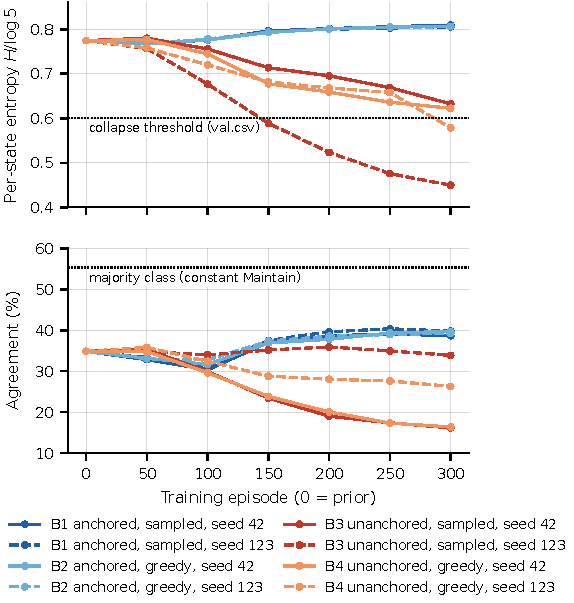
\includegraphics[width=\columnwidth]{figures/F2_val_trajectories}
\caption{Validation-split per-state entropy (top) and agreement (bottom) of the four Option~B arms at every 50-episode checkpoint, all five actors averaged, argmax selection; episode~0 is the shared prior. Dotted lines: the pre-registered collapse threshold on \texttt{val.csv} (0.60) and the majority-class agreement (55.3\,\%). No checkpoint was selected on these curves.}
\label{fig:f2_val}
\end{figure}

\begin{figure}[!t]
\centering
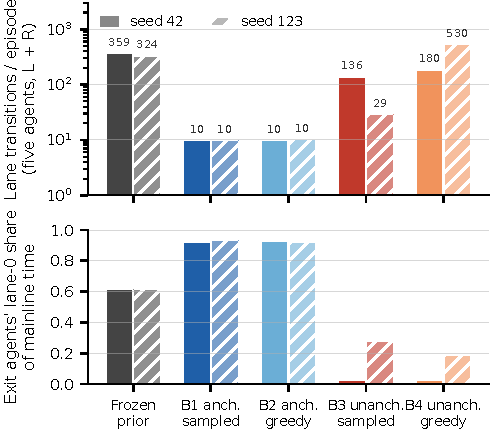
\includegraphics[width=\columnwidth]{figures/F3_lane_transitions}
\caption{Lane transitions per episode summed over the five agents, left and right, commanded and uncommanded (top, log scale), and the exit agents' share of mainline time spent in lane~0, the only lane that reaches the ramp (bottom), under mode~512 and sampled execution, 50 episodes per seed. The frozen prior of Section~\ref{sec:prior} is shown beside the four arms.}
\label{fig:f3_lanes}
\end{figure}

\begin{table*}[t]
\centering
\caption{Option B (protocol \S8.9--8.10): the same class-balanced prior fine-tuned for 300 episodes with and without the KL anchor, under sampled or greedy training action selection, two seeds, evaluated under \texttt{agent\_lane\_change\_mode=512} with both execution rules on matched episode seeds (50 per seed). Zero direct collisions and zero teleports in all 800 episodes.}
\label{tab:t5_option_b}
\footnotesize
\resizebox{\textwidth}{!}{%
\begin{tabular}{lcccccccc}
\toprule
\textbf{Evaluation execution: arm} & \textbf{$n$} & \textbf{Exit \%} & \textbf{Speed m/s} & \textbf{Prox./agent-km} & \textbf{$H$ per-state} & \textbf{$H$ selected} & \textbf{Exit agents' R moves: policy / SUMO} & \textbf{Lane-0 share} \\
\midrule
sampled: B1 anchored, sampled-trained, seed 42 & 50 & 85.3 & 11.9 & 37.4 & 0.714 & 0.723 & 280 / 0 & 0.95 \\
sampled: B1 anchored, sampled-trained, seed 123 & 50 & 80.0 & 11.2 & 41.0 & 0.706 & 0.717 & 278 / 0 & 0.95 \\
sampled: B1 anchored, sampled-trained, pooled & 100 & 82.7 & 11.6 & 39.2 & 0.710 & 0.720 & 558 / 0 & 0.95 \\
sampled: B2 anchored, greedy-trained, seed 42 & 50 & 85.3 & 11.8 & 38.3 & 0.720 & 0.730 & 282 / 0 & 0.96 \\
sampled: B2 anchored, greedy-trained, seed 123 & 50 & 69.3 & 10.4 & 44.5 & 0.707 & 0.718 & 278 / 0 & 0.95 \\
sampled: B2 anchored, greedy-trained, pooled & 100 & 77.3 & 11.1 & 41.4 & 0.713 & 0.724 & 560 / 0 & 0.95 \\
sampled: B3 unanchored, sampled-trained, seed 42 & 50 & 38.7 & 12.1 & 482.9 & 0.254 & 0.774 & 3299 / 1 & 0.21 \\
sampled: B3 unanchored, sampled-trained, seed 123 & 50 & 45.3 & 10.5 & 121.9 & 0.216 & 0.758 & 258 / 0 & 0.35 \\
sampled: B3 unanchored, sampled-trained, pooled & 100 & 42.0 & 11.3 & 316.7 & 0.235 & 0.766 & 3557 / 1 & 0.28 \\
sampled: B4 unanchored, greedy-trained, seed 42 & 50 & 41.3 & 12.6 & 425.2 & 0.236 & 0.766 & 4447 / 0 & 0.23 \\
sampled: B4 unanchored, greedy-trained, seed 123 & 50 & 35.3 & 10.6 & 102.8 & 0.310 & 0.928 & 13071 / 0 & 0.26 \\
sampled: B4 unanchored, greedy-trained, pooled & 100 & 38.3 & 11.6 & 276.2 & 0.273 & 0.847 & 17518 / 0 & 0.24 \\
\midrule
greedy: B1 anchored, sampled-trained, seed 42 & 50 & 100.0 & 24.5 & 8.3 & 0.650 & 0.010 & 278 / 0 & 0.96 \\
greedy: B1 anchored, sampled-trained, seed 123 & 50 & 100.0 & 24.5 & 8.2 & 0.636 & 0.014 & 277 / 0 & 0.97 \\
greedy: B1 anchored, sampled-trained, pooled & 100 & 100.0 & 24.5 & 8.3 & 0.643 & 0.012 & 555 / 0 & 0.97 \\
greedy: B2 anchored, greedy-trained, seed 42 & 50 & 100.0 & 24.5 & 8.3 & 0.666 & 0.020 & 278 / 0 & 0.96 \\
greedy: B2 anchored, greedy-trained, seed 123 & 50 & 100.0 & 24.5 & 8.2 & 0.658 & 0.013 & 277 / 0 & 0.97 \\
greedy: B2 anchored, greedy-trained, pooled & 100 & 100.0 & 24.5 & 8.3 & 0.662 & 0.017 & 555 / 0 & 0.97 \\
greedy: B3 unanchored, sampled-trained, seed 42 & 50 & 6.0 & 9.8 & 554.6 & 0.389 & 0.730 & 117 / 0 & 0.17 \\
greedy: B3 unanchored, sampled-trained, seed 123 & 50 & 30.7 & 9.2 & 116.2 & 0.271 & 0.756 & 135 / 0 & 0.29 \\
greedy: B3 unanchored, sampled-trained, pooled & 100 & 18.3 & 9.5 & 357.6 & 0.330 & 0.743 & 252 / 0 & 0.23 \\
greedy: B4 unanchored, greedy-trained, seed 42 & 50 & 6.0 & 9.8 & 619.5 & 0.370 & 0.704 & 2306 / 0 & 0.17 \\
greedy: B4 unanchored, greedy-trained, seed 123 & 50 & 23.3 & 9.4 & 161.8 & 0.461 & 0.931 & 9486 / 0 & 0.22 \\
greedy: B4 unanchored, greedy-trained, pooled & 100 & 14.7 & 9.6 & 409.3 & 0.415 & 0.817 & 11792 / 0 & 0.20 \\
\bottomrule
\end{tabular}}
\vspace{1mm}
\parbox{\textwidth}{\scriptsize Arms B1/B2 are anchored (CALM), B3/B4 unanchored, all from the identical prior checkpoint. The sampled rows are the primary comparison (the rule CALM trains with); under greedy execution B1 and B2 are the constant Lane\_Right policy.}
\end{table*}

\begin{table*}[t]
\centering
\caption{The pre-registered decision rule (protocol \S8.9 rev.~2) applied to B1 vs B3 under sampled execution and mode 512: primary $\Delta H_\mathrm{sim} \geq 0.10$ and $\Delta H_\mathrm{val} \geq 0.05$ on every seed; collapse $H_\mathrm{sim} \leq 0.50$ or $H_\mathrm{val} \leq 0.60$; guards by paired bootstrap over matched episodes within seed (10,000 resamples): exits difference lower bound $\geq -0.25$, proximity ratio upper bound $\leq 1.25$. Outcome: pass.}
\label{tab:t5b_decision}
\footnotesize
\resizebox{\textwidth}{!}{%
\begin{tabular}{lcccccccc}
\toprule
\textbf{Seed} & \textbf{$H_\mathrm{sim}$ B1} & \textbf{$H_\mathrm{sim}$ B3} & \textbf{$\Delta H_\mathrm{sim}$} & \textbf{$H_\mathrm{val}$ B1} & \textbf{$H_\mathrm{val}$ B3} & \textbf{Exits/ep B1 vs B3, 95\,\% CI of diff.} & \textbf{Prox./km B1 vs B3, 95\,\% CI of ratio} & \textbf{Primary / exits guard / prox. guard} \\
\midrule
seed 42 & 0.714 & 0.254 & 0.460 & 0.809 & 0.632 & 2.56 vs 1.16, [+1.12, +1.68] & 37.4 vs 482.9, [0.061, 0.100] & pass / pass / pass \\
seed 123 & 0.706 & 0.216 & 0.490 & 0.806 & 0.450 & 2.40 vs 1.36, [+0.70, +1.34] & 41.0 vs 121.9, [0.290, 0.385] & pass / pass / pass \\
\bottomrule
\end{tabular}}
\end{table*}


\subsection{Against the frozen prior}
\label{sec:prior}

The isolation above compares the anchored policy with a control that fine-tuning damaged. The control it does not include is the policy that was never fine-tuned. Table~\ref{tab:t6_frozen_prior} evaluates the Stage~0 class-balanced prior, loaded into all five agents exactly as the warm start installs it and left untouched, on the Option~B episode seeds under mode 512, and compares it with B1 and B2 by the paired bootstrap of Section~\ref{sec:contract_stats}. B1 was re-evaluated with its own step log for this comparison and reproduced its earlier summary metrics, per-episode records and per-seed entropies to the last digit; B2's per-episode entropies and lane transitions were lost to the step-log overwrite recorded in the table note and are reported from its per-seed summaries without intervals. No training was involved.

\paragraph{The prior as a policy.}
Under sampled execution the frozen prior exits 99.3\,\% of its exit agents at 11.9\,m/s with 46.9 proximity events per agent-km, per-state entropy 0.734 over its rollouts and selected-action entropy 0.886; its argmax spreads over Accelerate (39\,\%), Decelerate (25\,\%), Maintain (21\,\%) and the two lane changes (15\,\%), and its exit agents spend 71\,\% of their mainline time in lane~0. It does this while changing lanes about 340 times per episode over five agents---roughly the oscillation Section~\ref{sec:anchor} attributed to the unanchored arms---and under mode 512 those moves respect other drivers' gaps, so the oscillation costs it no exits. Under greedy execution it exits 69.3\,\% at 17.3\,m/s with 67.4 events per km. On the validation split it is the 34.85\,\% / 0.775 row of Table~\ref{tab:t4_val}.

\paragraph{Fine-tuning does not improve on it.}
Under the execution rule the anchored policy trains with, the prior matches or beats B1 on every declared measure. Per-state entropy over rollouts is slightly higher for the prior, 0.734 against 0.713 and 0.728 against 0.705, with intervals that exclude zero; the prior exits 2.98 agents per episode against 2.56 and 2.40, a loss of 0.42 and 0.58 exits per episode for CALM with intervals clear of zero; speed is indistinguishable ($+0.2$ and $-0.9$\,m/s, intervals crossing zero); proximity favours CALM on seed~42 (ratio 0.77, $[0.63,0.94]$) and is indistinguishable on seed~123 (0.91, $[0.76,1.07]$). Fig.~\ref{fig:f4_boot} shows the four bootstrap distributions for B1; B2 gives the same picture, with a larger exit loss on seed~123 (0.90) and a speed loss there ($-1.8$\,m/s). What fine-tuning measurably did is visible in the last column and in Table~\ref{tab:t4_val}: it removed the lane oscillation (340 to 10 transitions per episode), raised validation agreement by four points (34.85 to 38.7--39.8\,\%, still sixteen under the majority row), raised validation per-state entropy by 0.03 while lowering the simulator's by 0.02, and concentrated the argmax on Maintain and Lane\_Right (selected-action entropy 0.88 to 0.37). None of these is a gain on a declared measure under sampled execution.

\paragraph{Under greedy execution the comparison is between two different objects.}
Greedy B1 and B2 are the constant Lane\_Right policy of Table~\ref{tab:t3_gate}, which beats the greedy prior on exits (3.00 against 2.08 per episode), speed (24.5 against 17.3\,m/s) and proximity (ratio 0.12) at per-state entropy 0.64 against 0.74 and selected-action entropy 0.01 against 0.68. That advantage is the constant policy's, and it does not transfer to the stochastic policy CALM trains.

\paragraph{Consequence.}
``Anchoring prevents collapse'' stands as measured against the unanchored same-prior control. The stronger reading, that the fine-tuned anchored policy is better than its prior, is not supported under sampled execution on any declared measure: the anchored policy is the prior with its lane oscillation trained out, and nothing else measured was gained. In this benchmark the anchor is a regulariser that preserves, not one that improves, and more seeds could only tighten the intervals around no gain.

\begin{figure}[!t]
\centering
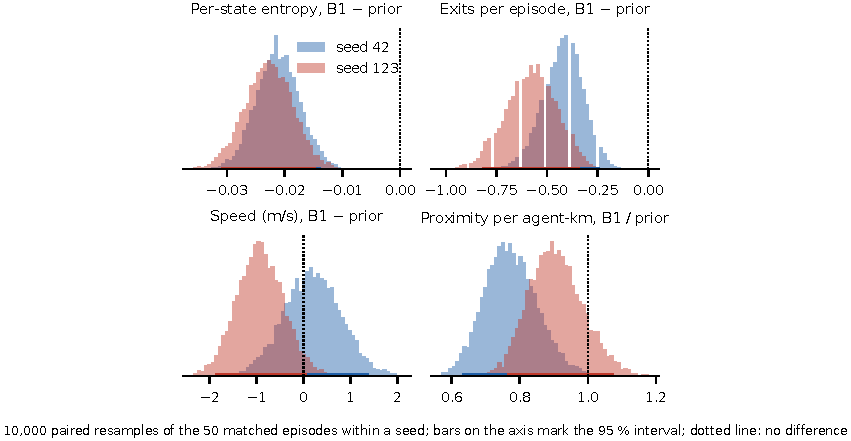
\includegraphics[width=\columnwidth]{figures/F4_paired_bootstrap}
\caption{Paired-bootstrap distributions of anchored B1 minus the frozen prior on the same 50 episodes within each training seed, sampled execution, mode~512: per-state entropy over rollouts, exits per episode, speed, and the ratio of pooled proximity rates. Three of the four intervals exclude no difference on both seeds in the prior's favour or at parity; proximity favours CALM on seed~42 only.}
\label{fig:f4_boot}
\end{figure}

\begin{table*}[t]
\centering
\caption{Anchored CALM against the frozen prior it was initialised from, on matched episodes (protocol \S8.11): the Stage 0 class-balanced prior loaded into all five agents and never fine-tuned, evaluated with the Option B episode seeds under mode 512. Differences are CALM minus prior with 95\,\% paired-bootstrap intervals over episodes within seed (10,000 resamples); proximity as the ratio CALM/prior of pooled rates.}
\label{tab:t6_frozen_prior}
\footnotesize
\resizebox{\textwidth}{!}{%
\begin{tabular}{lcccccc}
\toprule
\textbf{Execution: arm vs prior} & \textbf{$n$} & \textbf{$H$ per-state sim} & \textbf{Exits/ep} & \textbf{Speed m/s} & \textbf{Prox./km ratio} & \textbf{Lane changes/ep} \\
\midrule
sampled: B1 vs prior, seed 42 & 50 & 0.734 $\to$ 0.713, [-0.028, -0.014] & 2.98 $\to$ 2.56, [-0.62, -0.24] & 11.7 $\to$ 11.9, [-1.0, +1.4] & $\times$0.770 [0.631, 0.938] & 359 $\to$ 10, [-372, -327] \\
sampled: B1 vs prior, seed 123 & 50 & 0.728 $\to$ 0.705, [-0.031, -0.015] & 2.98 $\to$ 2.40, [-0.82, -0.34] & 12.2 $\to$ 11.2, [-1.9, +0.1] & $\times$0.905 [0.764, 1.074] & 324 $\to$ 10, [-337, -293] \\
sampled: B2 vs prior, seed 42 & 50 & 0.734 $\to$ 0.720$^\dagger$ & 2.98 $\to$ 2.56, [-0.62, -0.24] & 11.7 $\to$ 11.8, [-1.0, +1.2] & $\times$0.787 [0.647, 0.959] & 359 $\to$ 10$^\dagger$ \\
sampled: B2 vs prior, seed 123 & 50 & 0.728 $\to$ 0.707$^\dagger$ & 2.98 $\to$ 2.08, [-1.18, -0.64] & 12.2 $\to$ 10.4, [-2.7, -0.9] & $\times$0.984 [0.856, 1.135] & 324 $\to$ 10$^\dagger$ \\
\midrule
greedy: B1 vs prior, seed 42 & 50 & 0.743 $\to$ 0.649, [-0.102, -0.085] & 2.08 $\to$ 3.00, [+0.84, +0.98] & 17.4 $\to$ 24.5, [+6.3, +7.8] & $\times$0.125 [0.110, 0.143] & 259 $\to$ 10, [-269, -232] \\
greedy: B1 vs prior, seed 123 & 50 & 0.739 $\to$ 0.636, [-0.114, -0.091] & 2.08 $\to$ 3.00, [+0.84, +0.98] & 17.3 $\to$ 24.5, [+6.4, +8.1] & $\times$0.120 [0.103, 0.143] & 248 $\to$ 10, [-254, -223] \\
greedy: B2 vs prior, seed 42 & 50 & 0.743 $\to$ 0.666$^\dagger$ & 2.08 $\to$ 3.00, [+0.84, +0.98] & 17.4 $\to$ 24.5, [+6.3, +7.8] & $\times$0.125 [0.110, 0.143] & 259 $\to$ 10$^\dagger$ \\
greedy: B2 vs prior, seed 123 & 50 & 0.739 $\to$ 0.658$^\dagger$ & 2.08 $\to$ 3.00, [+0.84, +0.98] & 17.3 $\to$ 24.5, [+6.4, +8.0] & $\times$0.120 [0.104, 0.142] & 248 $\to$ 10$^\dagger$ \\
\bottomrule
\end{tabular}}
\vspace{1mm}
\parbox{\textwidth}{\scriptsize $^\dagger$B2's per-episode step log was overwritten by a later arm (protocol \S8.10 caveat); its entropy and lane changes are the per-seed summary values without an interval. B1 was re-evaluated with its own log, identical to the 4 November run. Under sampled execution the prior has equal-or-higher per-state entropy, more exits and the same speed; proximity favours CALM on seed 42 only. Under greedy execution B1 and B2 are the constant Lane\_Right policy (Table~\ref{tab:t3_gate}).}
\end{table*}


\subsection{Training reward, labelled}
\label{sec:reward}

The hybrid training reward is the quantity the submitted paper reported as ``final reward'' and ranked methods by. The evaluator returns no reward, so nothing in Tables~\ref{tab:t2_table3}--\ref{tab:t6_frozen_prior} is a reward, and no reward figure in this paper is an evaluation outcome. For the record, the mean reward over the last 50 training episodes, with exploration and under each arm's training rule, was 1.39 and 1.35 for B1, 1.26 and 1.23 for B2, 0.87 and 0.70 for B3 and 0.86 and 0.74 for B4 (Fig.~\ref{fig:f5_reward}), and in the pilot 1.42 and 1.50 for class-balanced CALM against 1.28 and 1.31 for CALM on the unweighted prior. The anchored arms' higher reward is consistent with their exits and proximity relative to the unanchored arms, and the reward charges each lane change, so part of the gap is the oscillation itself; but the pilot ordering runs against the evaluator---the unweighted-prior policy that reward ranks lower was, under SUMO's default mode, the policy with the most exits, the highest speed and the fewest near-misses---and the frozen prior, which has no training reward at all, matched or beat every anchored arm under sampled execution. A training statistic measured under exploration noise, on the training environment's own episodes, is not a measurement of the deployed policy, and we report it only as what it is.

\begin{figure}[!t]
\centering
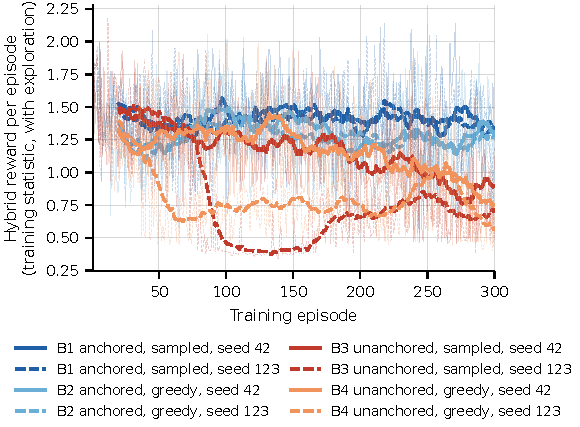
\includegraphics[width=\columnwidth]{figures/F5_training_reward}
\caption{Hybrid training reward per episode for the four Option~B arms and both seeds (faint: raw log; solid: 20-episode moving mean), with exploration and under each arm's training selection rule. A training statistic that the evaluator does not measure; no table in this paper uses it.}
\label{fig:f5_reward}
\end{figure}
